\chapter{Aufbau \sppname}

\section{Architekturbeschreibung}

Sinn und Zweck dieses \gls{snort} \gls{praeprozessor}s \gls{sppname} ist das Abfangen,
Komprimieren und Weiterleiten von \gls{profinet}-\glspl{paket}n. Diese
sind am \gls{ethertype} erkennbar. Er muss der Hexadezimalzahl 0x8892 entsprechen.
Hauptbestandteil des \gls{praeprozessor}s ist eine erweiterbare Baumstruktur von Decodern, welche rekursiv, Schicht für Schicht, ein \gls{paket} bearbeiten und die Informationen, die wir haben wollen, in ein Truffle schreiben. Ein Truffle ist eine von uns vordefinierte Datenstruktur im \gls{praeprozessor}.
Pro Netzwerk-\gls{paket} entsteht also ein Truffle, welche erheblich kleiner und kompakter als herkömmliche Netzwerkpakete sind. Dieses wird dann über den \gls{ipc}-Teil des \gls{praeprozessor}s
an unser \gls{programname} versendet um den Informationsfluss zu erhalten aber auch zu minimieren.\newline
Jetzt kommt die Sicherheit ins Spiel. Wir können zusätzlich mit einer von uns selbst geschriebenen Datenstruktur ab diesem Zeitpunkt des Informationsflusses für einiges mehr an Sicherheit garantieren.
Ein weiterer Vorteil der Truffles ist die Gelegenheit für einen Sicherheitscheck bevor es gesendet wird. Wir wissen aufgrund der rekursiven Struktur unseres Decoder-Baums welche Daten wir zu erwarten haben. Sollte wir Inkonsistenzen feststellen, es ein Fehler vorliegen, oder etwas anderes keinen Sinn ergeben, so setzen wir im Truffle entsprechende Flags, damit \gls{programname} Statistik für Auffälligkeiten einzelner Kommunikationsteilnehmer führen kann.\newline
\gls{sppname} ist absichtlich klein gehalten, da es empfohlen wird diese \gls{snort}-\gls{praeprozessor}en nicht performance-lastig zu entwerfen. Der oben beschriebenen Ablauf findet sich als Sequenzdiagramm in Kapitel 4.


\section{UML-Diagramm}

\begin{sidewaysfigure}
  \centering
  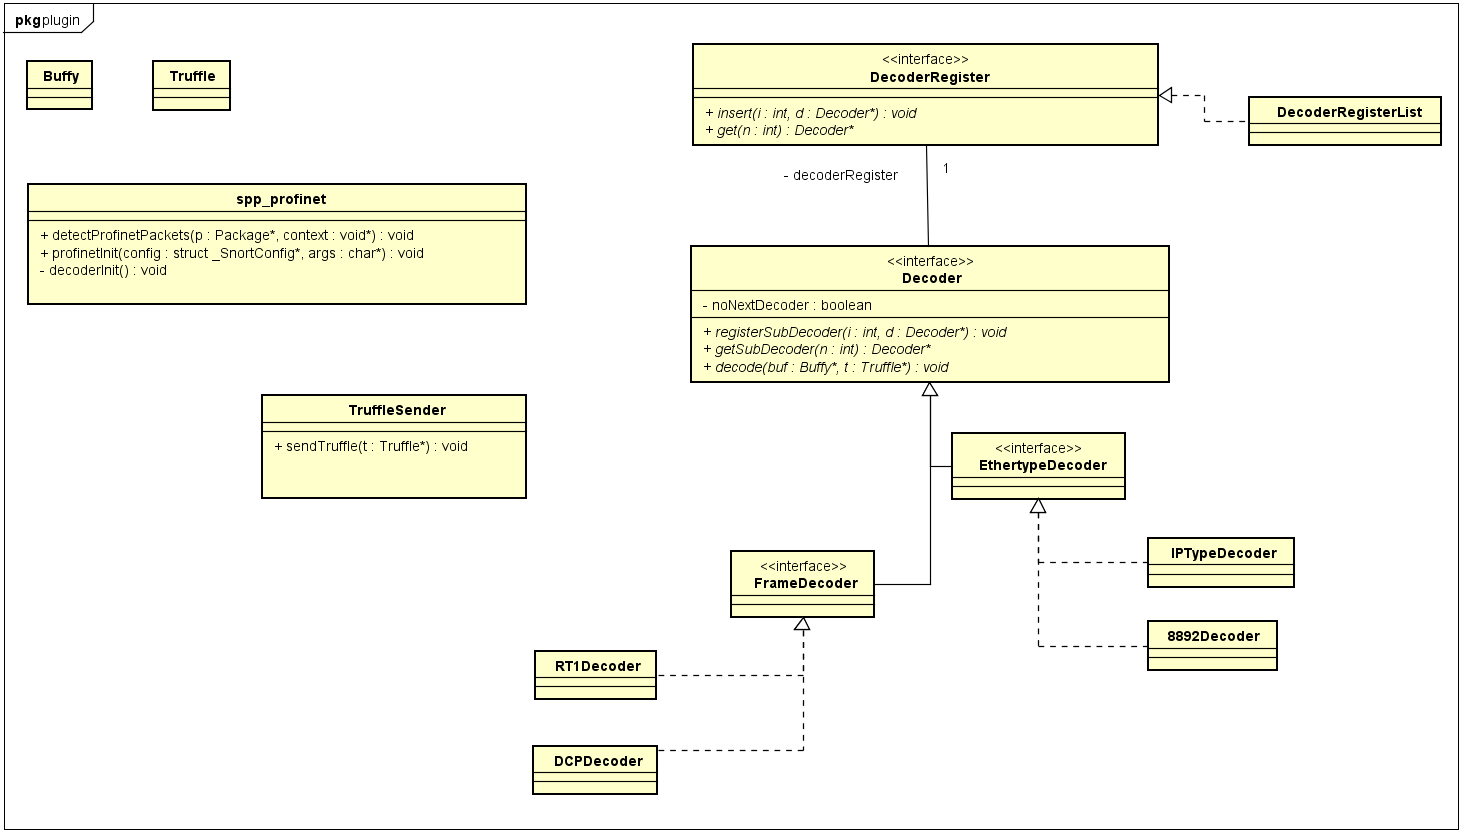
\includegraphics[width=\paperwidth]{../diagramimages/spp_profinet.png}
  \caption{\gls{praeprozessor} \gls{sppname}}
\end{sidewaysfigure}
